\section{Discussion}

\subsection{Nitrite Investigations}
From our experimentation, we have found that use of both disposable and reusable gold electrodes are suitable for measuring nitrite concentrations in solution. Our chosen nitrite concentrations reflect the normal physiological levels and expected elevation in septic patients. DPV is a reliable method of measuring the electrochemical activity of nitrite in solution. However, using our parameters, each measurement takes 405 seconds, which may prove a challenge in a clinical setting, as well as in the context of real-time monitoring. 

One challenge faced during experimentation was the pHEMA coating applied to the RE on the disposable gold electrode. We found that during DPV, the pHEMA layer was insufficient to prevent reaction on the RE, thus resulting in destruction of the electrode. As a result, frequent replacement of the disposable electrode was required. In a clinical context, this is non-ideal, as replacement of electrodes is more expensive, creates more waste and is less practical for clinicians and patients. Potential solutions for this issue are applying a thicker coating of pHEMA onto the RE or using a different compound entirely. However, these may also change the electrochemical properties of the electrode. 

DPV voltammograms from nitrite experimentation reveals a common peak where the peak current recorded increases with higher concentrations of nitrite, across all experiments, between 0.7 and 0.8 V, which is expected from literature \cite{article} Small peaks corresponding to an unknown species was reliably detected at 0.2 V in PBS only experiments, but were not present in albumin experiments. This may be due to the increased noise and smoothing eliminating this peak. We hypothesise that small peaks may be due to oxygen impurities in solution. 

From our albumin experiments, it is interesting that at low nitrite concentrations (below 16 µM), the sensitivity is comparable to our results without albumin. However, at higher nitrite concentrations, the sensitivity increases to 7nA µM-1, with a marked change in the calibration curve (Figure 8), suggesting interactions between the nitrite and the albumin. 

Detected current was also overall greater in albumin experiments vs without albumin. These results seem to contradict the hypothesis that albumin precipitates onto the surface of the electrode, as we would expect lower values. 


\subsection{Hydrogen Peroxide Investigations}
To perform hydrogen peroxide electrochemical detection using the microneedles platform, we have conducted chrono amperometry, an electrode calibration experiment, with gold electrodes over a range of hydrogen peroxide concentrations. The calibration process was facilitated by hydrogen peroxide and Prussian blue reactions. Following the amperometry, we performed coulometry to validate the experimental concentration and amplify the signal and reduce the noise from the raw data. \\\\It is observed that under low hydrogen peroxide concentrations, specifically below 100uM, there are significant percentage differences between the experimental and theoretical concentration values. In the future, a more discreet selection of the equipment for liquid transferring is critically required, thus an improvement of the experimental accuracy can be accomplished. Also, a non-linearity condition was observed in the current vs time plot under high hydrogen peroxide concentrations, especially when $c>300$uM. By performing quantitative analysis based on \autoref{eqn:h2o2redox1},  \autoref{eqn:h2o2redox2} and the actual amount of reactants involved in the experiment, an approximation of hydrogen peroxide concentration limit was found at 280uM, indicating an excess of the hydrogen peroxide concentration would result in insufficient PB to react with H$_{\text{2}}$O$_{\text{2}}$. 


\subsection{Lactate Investigations}
The differences in behaviour of the current concentration behaviour conveyed in \autoref{fig:lactate_result}(b) and (c), can be explained by the enzyme kinetics of the lactate oxidase.\\\\
The linear range suggested by the data is 0.0-2.0mM/L lactate- here, the current is approximately purely dependent on the concentration of lactate. The flow of electrons is indicative of the rate of reaction and in this region of the graph the concentration of enzyme or enzyme ability to allow binding has no effect on the sensing abilities. After 2.0mM/L the rate of reaction can be seen as starting to plateau, whilst there is no limit in detection observed in the range of concentrations tested, it can be assumed that it is being approached. The non-linear behaviour of the relationship is therefore due to enzyme kinetics.  
\begin{figure}[H]
    \centering
    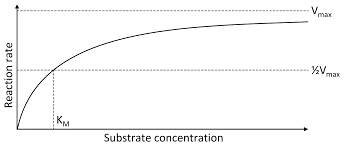
\includegraphics{img/lactate_discussion_1.png}
    \caption{Michaelis-Menten Kinetic plot of enzyme substrate reactions. }
    \label{fig:lactate_discussion}
\end{figure}
Michaelis Menten equations for reaction velocity \cite{johnson2011original}:
\begin{equation}
    E + S \xrightleftharpoons[k_{\text{off}}]{k_{\text{on}}} ES \xrightarrow{k_{cat}} E+P \quad \quad v = \frac{V_{max}[S]}{K_{M}+[S]}
\end{equation}
Enzyme kinetics can be defined partially by their Michaelis- constant Km which describes the concentration of lactate at which the current is half of that of the detection limit as seen in \autoref{fig:lactate_discussion}. In the Michaelis- Menten model, $v$ represents the velocity of the reaction, in this experiment we can take the current to be proportional to $k_{cat}$, and hence proportional to the velocity of the H\textsubscript{2}O\textsubscript{2} production. We can see from the Michaelis-Menten equation, since $V_{max}$ and Km are constants the plot is hyperbolic, at higher concentrations, we can expect a decreased climb in velocity which our calibration plot is in accordance with. Since Michaelis-Menten kinetic models would require that immobilisation of the LOX in the matrix have no effect on its affinity for lactate, we instead approximate a value for $K_{m}$ by calculation an apparent constant $K_{m[app]}$.  It is not possible to determine exactly this value since $V_{max}$ cannot be observed in this range however we can approximate the maximum current to be around $5.5\times10^{-6}$ A based on our calibration curve. This would then give a $K_{m[app]}$ proportional to the concentration where a current of $2.75\times 10\textsuperscript{-6}$A would be observed, approximately 1.2mM.\\\\
We can conclude that the sensor is therefore useful at detecting concentrations in the range experimented. Although readings plateau in the upper range of lactate concentrations, since a patient is septic anywhere in this range- the same measures (i.e administration of antibiotics) would be taken whether the patient exhibits levels in the 3.5-4.5mM/L range as would be taken if levels are beyond 4.5mM/L.  
\subsection{Aptamer Modelling}
In this study, we have developed a novel numerical inverse laplace algorithm capable of decomposing multi-exponential chronoamperometric current signals. We show this algorithm is able to resolve rate constants up to a resolution of $k_{A} = 200s^{-1}$ and $k_{AT} = 400s^{-1}$, with simulated signals with realistic noise levels. These values of rate constants are closer compared to the $k_{A} = 125s^{-1}$ and $k_{AT} = 500s^{-1}$ quoted in Plaxco's study \cite{arroyo2018subsecond}.\\\\
In parallel, we develop a coarse-grained model of aptamers by assuming it as a freely-jointed chain to gain insight into the physical effects of target binding. We generate length probability distributions, and assess how the probability of a collision event $P(L<1.5nm)$ varies with Aptamer length.\\\\